\chapter{Design of Demo Devices}
This chapter is focused on the tag reader and power control device of the \textbf{Parentsystem}. 
The design and functionality of the prototype will be presented in parallel to the designed end product.

\section{Product Design}

There is two devises need to activete a usage of device from the user to the server as shown in figure below.

\begin{figure}[h]
	\centering
		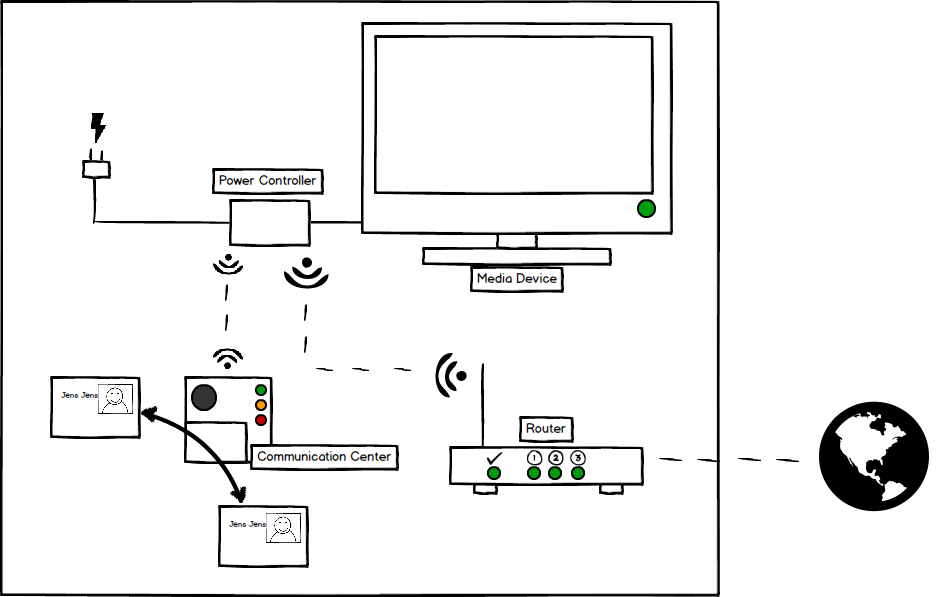
\includegraphics[width=1.00\textwidth]{C:/Users/JML88/Documents/GitHub/MOM/report/images/Power&Tagdevice.png}
	\caption{Rich picture for Powercontrol and Tag reader}
	\label{fig:Power&Tagdevice}
\end{figure}

One is a small detection device to read user tags when swiped over it, this devise is often placed in the most asseble place. 
The other devise is a powercontrol devise whitch i located on the powerline to the media device and tunes on and off the electrisity when needed.
The powercontrol devise(PCD) is the brain of the two devises and is therefore to moniter the users time usage and communication center with the server and detection devise. 
The detection devise(DD) also work as infomation communicater to the user on the state of the connection to the server, acceptens/decline of login and more.     

\subsection{Senario Design}

The systemt is designed on mulitble senarios and the creteria of communication to server and user. The flow chart below is a overview of actions and communication the two devices have to give the right permission to user, communicat with the user and server about status, handel disconnection to server and control of user- and timeusage restrictions.

\fixme{indsæt Flowcart af systemet}

To test develop the flowcart of the system is multible usercases constucted.

\textbf{Setting up and turning on the system.} \n
The PCD retive information on wifi connection form USB port if an USB is connected at start point of PCD. 
If the USB information is wrong or not retived then a restart botton is included to redo the procedure.  \n
The PCD will then connect to the wifi network and to the web server of MOM. If the connection isn't found a massage is send to the DD. \n DD indicate that there is no connection by blinking the red light \fixme{indsæt referance til appendix table af lys indikater}.\n When the connection is established then the server will communicate what state the media device should be in. If it is open to for usage then the DD will blink a orange light else constant red light and a blinking orange light. 

\textbf{Detection of connection issues and waiting for tag.} \n
The connection to the sever is tested by a rutine call every five minutes form the PCD to the server. In the meanwhile will the PCD ask for a tag from the DD which blick the orange light. If the PCD is disconnected form the server at the rutine call the DD will again light a constant red and a blinking orange.    
  
\textbf{Logon/logoff media divice.} \n
When a tag is read by the DD will the PCD recieve the tag id which formed to a login massage if no one is all ready logged in the system. The PCD will then read if the user is declined or accepted to use the device. If the user is declined to use the divece then will the DD blink three times with the red light. If the user is accepted then the PCD will switch the power on to the media device, save the tag id in local memory and recieve time left before a rule or to time usage limit accour. The DD indicate that the user i approve to use the media device with a constant green light.\n When the PCD recieve the tag id that is stored in the local memory then it means the user is logging off. The PCD will switch off the poer to the media device and send a logoff massage til the server. The DD will return to only blink the orange light. Should another user want to take over the usage of a media device the PCD will try to login with the new tag if declined then the DD will blink the red ligh 3 times else if accepted then the server will overwirte the the previus user and PCD will recieve the information for the new user and the DD will blink with the green light 3 times.

        

The standard user senario:
The tag dectector reads the identification tag when the user swip it on the device and sends the information to the powercontorl device with a low frequency connection.
The powercontrol device translate the swip to a command that is send to the server with the devise id and tag id. The server will respond, if the user is allowed to use the media then the powercontroler turn on the powersupplie else it dosn't in both cases it gives the information to the tag detector to confirm/decline the logon to the user though it's indications lights and time that is able before a rule or time barrier sets in visa versa for logging off the system(light indications is descriped in table XXXX). It is possible for the system to let a other user to take over media divice when swiping his/her tag and the previus user is logged off and the the new logged in without turning the powersupply of. ofcouse this is only if the user i allowed on the media device. 

Time- and user restriction senario:
A user may end up using all the time whitch is given or incounter a rule that will shout off the devise. The powercontroler as communicat to the server every five minuts to get updates. This call to the sever is both to insure that there is a connection and for any changes to the allowed usage for the current user. To avoid that the media devise suddenly is shout down due to a restigtion or the user time is used up a five min warning is send from powercontroler to the detection devise to the user though the small speaker. 

These two senarios is not always the reallity because of connection malfunction. 
This "`apnormalties"' creates design quistions that will influens the user in one way or the other.   
Lost of connection is decovered when there is no connection at a status call that is send every five min form the powercontrol devise. With this rutine the server know that it has lost connection with the devise when it haven't resieved and massage in five miniuts. The user will see on the detector device that there is no connection. If the connection lost at a time when the user is using the media devise the light indicate this and keep the media devise turned on. The powersupply devise will still keep track af the timeusage and user restrigtions. If the user logoff the media devise then the powercontrol devise set a timestamp whitch is send to the server then the connection is reastablage. The lost connection on the server side consider it as the user has logget off within the last five miniuts. This procedure have the advange that the user will not have to cut off the media in use if the connection is waopely and the user will be able to login on other media device even with previus media divice not yet have connection. The disavenge is that the user has the possiblety to overuse the time resigtion by still use the disconnected divice until there is no more time and in the mean time has turned on at new device. The disadvange will but also have the effect to punish the user with a big negitive time to use other devices when the disconnected device is reconnected and this should discourage this senario. 

\section{Prototype Implemtation}
The prototype is designed to prove the concept of a tag reader and the communication protecal between powercontrol and server. Therefor shall the Ardurino hardware be seen as replaceble for to manufature this system it is need be unic devices that is able to connect on the power core to the the media device and slim designed card reader with speaker and indications lights. To prove the conecpt the device is able to read and accept/decline tags, indicate this using ligts to the user and turn on the power if accepteted.   

    